\section{Implementation}\label{sect:implementation}
We have now provided a brief history of objective video quality assessment, explained the various approaches one may take in assessing video quality and provided reasoning for choosing the standardized model we have. In this section we will explain the decisions made with regards to the implementation itself. We will also present the current progress of our implementation, and talk about the work laying ahead of us.

\subsection{Coding decisions}\label{sect:coding}
Since the PEVQ model from ITU-T Rec. J.247 is designed for resolutions up to VGA we hope to have the opportunity to further develop and test the implementation to support high definition resolutions. 
As we want to focus on the PEVQ implementation itself rather than the video handling surrounding it, it is important to choose the shortest path towards writing PEVQ implementation code. Being able to not create a whole framework for video decoding, encoding, writing etc will save us a lot of valuable time. This may also provide us with the time to further build on the PEVQ model to support resolutions higher than VGA in the future. in order to skip this step we have decided to use the open source library, Libav\cite{libav} which allows us to start implementing algorithms from PEVQ immediately after setting up an environment for Libav.

Libav is a C library with bindings to several other languages, but as the algorithms in PEVQ require a high amount of computing power it is essential to choose a coding language where high performance is possible. Writing the implementation in C or C++ was therefore a natural choice, whereas we have decided to focus on C++ to create a modern and object oriented solution.

We would also like to briefly mention the possibility of porting the program to a graphics processing unit (GPU). While this is not part of the initial plan, we are aware of the speedup possibilities that lie within GPU execution when dealing with image or video processing the way we are. One of the more computing intensive parts of the PEVQ solution is the calculation of the edge images using a Sobel Filter. A demonstration of speedup gained when executing a Sobel edge filter on a GPU rather than a CPU can be viewed in a paper by A. Dore and S. Lasrado in\cite{sobelFilterGPU}. Allowing users to run the video quality assessment tool faster will surely be an appreciated feature.

As may be interpreted from section~\ref{sect:pevq}, the PEVQ model itself is somewhat modular. Each step is more or less standalone, relying on the results from a previous step in varying degrees. Before the actual quality assessment can be performed, the model makes sure the source and degraded signal are aligned properly. This is so that when comparing results the comparison is done between the correct parts of the video in case the degraded signal has been stretched in any way. Should the analysis stage learn that the video sequences are satisfactory aligned, the alignment module of the code can be skipped. 
We will design our solution in such a way that if the assessment tool detects something which can be skipped, it can proceed with the next step and get a performance gain.

\subsection{Preliminary results}\label{sect:results}

So far we have been able to implement code for the pre-processing and signal analysis stages, in addition to Libav specific code to handle loading, encoding, decoding and writing of video files to disk. This means we are able to load any video file, decode it into a YUV format we can work with in our PEVQ implementation, for later to write video sequences for testing purposes to disk. We have also created simple data dumping for values created in the signal analysis stage which allows us to control the results. 

\begin{figure}[h]
	\centering
	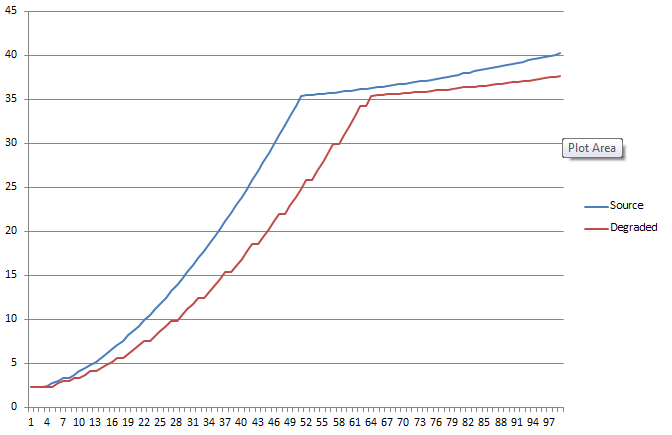
\includegraphics[width=.7\textwidth,natwidth=672,natheight=435]{images/stdDevEdgeImg.png}
	\caption{Source and degraded standard deviation edge image.}
	\label{fig:stdDevEdgeImg}
\end{figure}

Figure~\ref{fig:stdDevEdgeImg} visualizes the values from the standard deviation of the Sobel Filter edge image. In this test we used a source video sequence at 24 frames per second and a degraded signal at 30 frames per second. We see that the degraded signal is lagging behind the source signal more and more, and that the standard deviation value is completely similar for two consecutive frames each time the degraded signal seems to be additionally delayed. While this is just a small part of the PEVQ model, the standard deviation from the edge image, among other results, is used to perform the coarse temporal alignment as described in section~\ref{sect:pevq}. The result from figure~\ref{fig:stdDevEdgeImg} clearly illustrates that the video sequence will need some sort of temporal alignment in order for the two video sequences to be properly aligned. If such an alignment is not performed, further analysis on a frame by frame basis will not match in the time domain.  With regards to what we talked about in section~\ref{sect:coding}, this discovery translates to the fact that we need to run the alignment module. 
